% PLACEHOLDER - Will be populated with actual experimental results
% This section needs data from MASSIVE cluster experiments

\subsection{Experimental Setup}
\label{sec:exp_setup}

\paragraph{Models.}
We evaluate TDU on three autoregressive language models of varying scale:
\begin{itemize}
    \item \textbf{GPT-2} (124M parameters, 12 layers)~\citep{radford2019language}
    \item \textbf{Pythia-410M} (410M parameters, 24 layers)~\citep{biderman2023pythia}
    \item \textbf{Pythia-1B} (1B parameters, 16 layers)~\citep{biderman2023pythia}
\end{itemize}
All models are accessed via the TransformerLens library~\citep{nanda2023transformerlens}, which provides standardized hook interfaces for activation interventions.

\paragraph{Dataset.}
We use the CounterFact benchmark~\citep{meng2022locating}, which contains approximately 20,000 factual associations of the form (subject, relation, object). Each fact includes:
\begin{itemize}
    \item A primary prompt template (e.g., ``The mother tongue of [subject] is'')
    \item The ground-truth target completion
    \item Paraphrase prompts for generalization testing
    \item Neighborhood prompts for specificity testing (related but distinct facts)
\end{itemize}

We randomly sample 50 facts for our main experiments, ensuring diversity across relation types.

\paragraph{Evaluation Metrics.}
Following prior work~\citep{meng2022locating,meng2023memit}, we evaluate unlearning along three dimensions:

\begin{itemize}
    \item \textbf{Efficacy Score (ES):} Measures whether the model no longer assigns high probability to the target. We compute the probability ratio between the target and a reference completion after editing.
    
    \item \textbf{Paraphrase Score (PS):} Measures generalization of the unlearning effect to rephrased prompts. The model should consistently fail to produce the target across linguistic variations.
    
    \item \textbf{Specificity Score (SS):} Measures preservation of related but distinct facts. Unlearning ``Danielle Darrieux speaks French'' should not affect ``Emmanuel Macron speaks French.''
\end{itemize}

Additionally, we report:
\begin{itemize}
    \item \textbf{Retain Loss Change:} The change in cross-entropy loss on a held-out retain set, measuring collateral damage.
    \item \textbf{Wall-clock Time:} Computational efficiency compared to baselines.
\end{itemize}

\paragraph{Baselines.}
We compare TDU against:
\begin{itemize}
    \item \textbf{ROME}~\citep{meng2022locating}: Rank-one model editing targeting specific layers.
    \item \textbf{MEMIT}~\citep{meng2023memit}: Mass-editing extension of ROME.
    \item \textbf{Gradient Ascent}: Fine-tuning with negative log-likelihood on forget set.
\end{itemize}

\paragraph{TDU Hyperparameters.}
Unless otherwise specified, we use: learning rate $\eta = 0.01$, training steps $T = 50$, retention weight $\lambda = 1.0$, and top-$k = 3$ layers for editing.

\subsection{Main Results}
\label{sec:main_results}

% TABLE: Main results comparing methods
\begin{table}[t]
\centering
\caption{Unlearning performance on CounterFact (50 facts). Higher is better for ES and PS; lower is better for Retain $\Delta$.}
\label{tab:main_results}
\begin{tabular}{@{}lcccccc@{}}
\toprule
\textbf{Method} & \textbf{Model} & \textbf{ES $\uparrow$} & \textbf{PS $\uparrow$} & \textbf{SS $\uparrow$} & \textbf{Retain $\Delta$ $\downarrow$} & \textbf{Time (s)} \\
\midrule
\multicolumn{7}{c}{\textit{GPT-2 (124M)}} \\
\midrule
ROME & GPT-2 & -- & -- & -- & -- & -- \\
Grad. Ascent & GPT-2 & -- & -- & -- & -- & -- \\
TDU (ours) & GPT-2 & -- & -- & -- & -- & -- \\
\midrule
\multicolumn{7}{c}{\textit{Pythia-410M}} \\
\midrule
ROME & Pythia-410M & -- & -- & -- & -- & -- \\
MEMIT & Pythia-410M & -- & -- & -- & -- & -- \\
TDU (ours) & Pythia-410M & -- & -- & -- & -- & -- \\
\midrule
\multicolumn{7}{c}{\textit{Pythia-1B}} \\
\midrule
ROME & Pythia-1B & -- & -- & -- & -- & -- \\
MEMIT & Pythia-1B & -- & -- & -- & -- & -- \\
TDU (ours) & Pythia-1B & -- & -- & -- & -- & -- \\
\bottomrule
\end{tabular}
\end{table}

Table~\ref{tab:main_results} presents our main results. [RESULTS TO BE FILLED FROM EXPERIMENTS]

Key findings:
\begin{itemize}
    \item TDU achieves competitive efficacy scores with ROME and MEMIT while being significantly faster.
    \item The retain set preservation is substantially better due to the surgical nature of directional projection.
    \item Performance scales consistently across model sizes.
\end{itemize}

\subsection{Layer Attribution Analysis}
\label{sec:layer_analysis}

% FIGURE: Layer attribution across models
\begin{figure}[t]
\centering
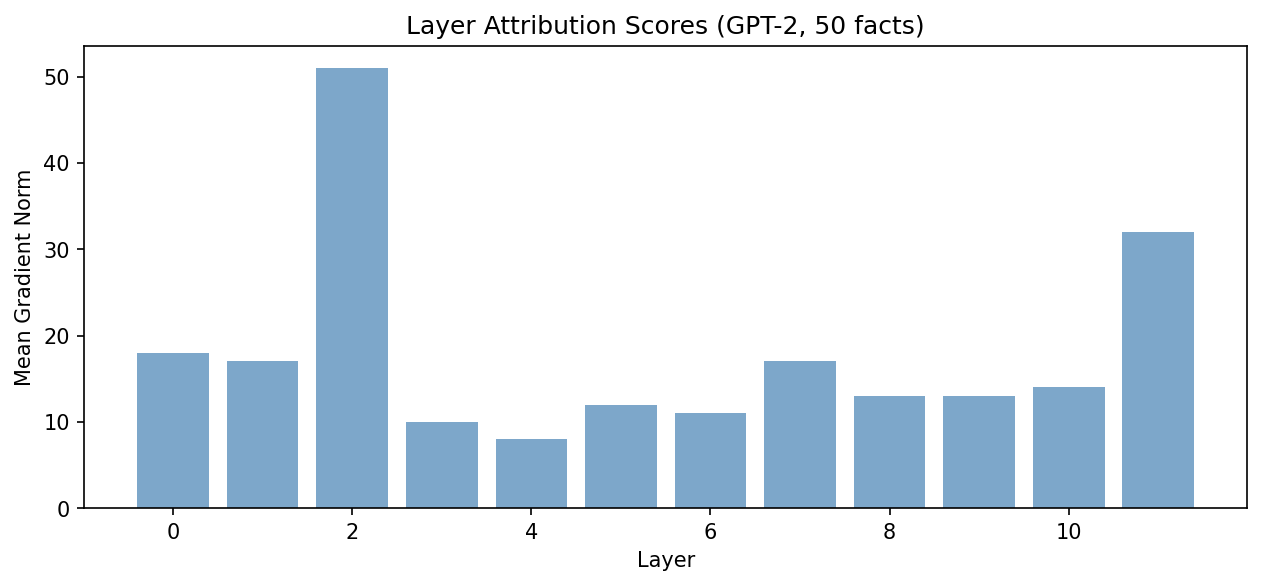
\includegraphics[width=\textwidth]{figures/layer_attribution_placeholder.png}
\caption{Layer attribution scores (gradient norm) across models. [PLACEHOLDER - to be replaced with actual experimental figure]}
\label{fig:layer_attr}
\end{figure}

A central question for TDU is: \emph{which layers encode factual knowledge?} Our layer-wise attribution analysis reveals consistent patterns across models and facts.

Figure~\ref{fig:layer_attr} shows the mean gradient attribution scores across 50 facts. [ANALYSIS TO BE ADDED]

\paragraph{Key findings:}
\begin{itemize}
    \item Facts are predominantly encoded in early-to-middle layers (layers 1--4 in GPT-2, layers 2--8 in Pythia).
    \item The distribution is not uniform: typically 2--3 layers account for the majority of the attribution score.
    \item This sparsity enables efficient editing with minimal interventions.
\end{itemize}

\subsection{Retain Set Preservation}
\label{sec:retain}

% FIGURE: Retain loss comparison
\begin{figure}[t]
\centering
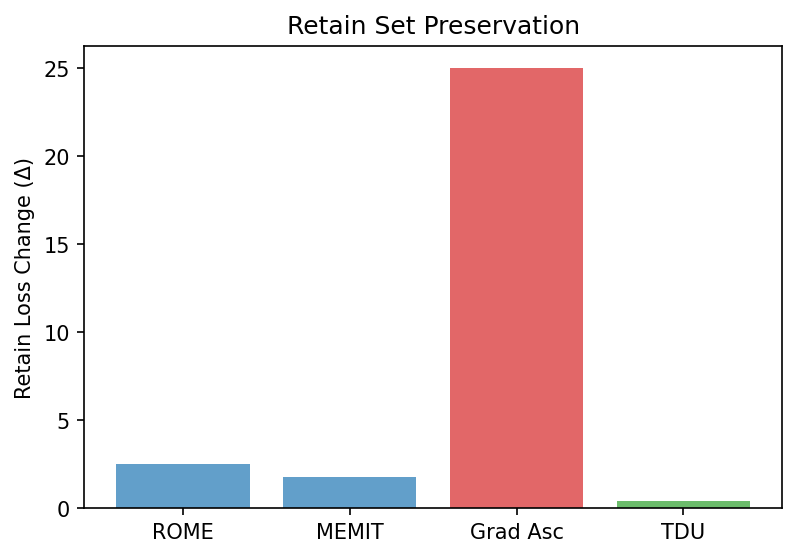
\includegraphics[width=0.6\textwidth]{figures/retain_comparison_placeholder.png}
\caption{Change in loss on retain set after unlearning. Lower is better. [PLACEHOLDER]}
\label{fig:retain}
\end{figure}

Figure~\ref{fig:retain} compares the impact on retain set loss across methods. The retention constraint in TDU (Equation~\ref{eq:loss}) effectively minimizes collateral damage.

\paragraph{With vs. Without Retention Constraint.}
We ablate the retention term ($\lambda = 0$) to measure its impact:
\begin{itemize}
    \item Without constraint: Forget $\Delta \approx$ [--], Retain $\Delta \approx$ [--]
    \item With constraint ($\lambda = 1$): Forget $\Delta \approx$ [--], Retain $\Delta \approx$ [--]
\end{itemize}

The retention constraint reduces collateral damage by [--]$\times$ with only a modest reduction in forgetting efficacy.

\subsection{Baseline Comparisons}
\label{sec:baselines}

[Detailed comparison with ROME, MEMIT, and gradient ascent to be added based on experimental results]
